\documentclass{tietreport}

% Import images
\usepackage{graphicx}

% Tables with wrapped text columns
\usepackage{array}
\newcolumntype{L}[1]{>{\raggedright\arraybackslash}p{#1}}

% Bibliography configuration
\usepackage[
  date=year,
  style=alphabetic,
  backend=biber,
  sorting=nty,
  maxnames=5,
  minnames=3,
  maxalphanames=4,
  minalphanames=3,
  backref=true,
  doi=false,
  isbn=false,
  url=false,
  eprint=false
]{biblatex}
\addbibresource{references.bib}

% Every figure quoted below, generated from the repository's data
% by scripts/final_report_figures.py
% Written by scripts/final_report_figures.py. Do not edit.
\newcommand{\SnapshotDate}{21 November 2026}
\newcommand{\TableRows}{631}
\newcommand{\FirstReading}{19 February 2025}
\newcommand{\DataAvailability}{90\%}
\newcommand{\ValidDays}{576}
\newcommand{\SpanDays}{641}
\newcommand{\ValidShare}{90\%}
\newcommand{\BtFirst}{3 April 2025}
\newcommand{\BtLast}{21 November 2026}
\newcommand{\BtDays}{485}
\newcommand{\RefAge}{2}
\newcommand{\MaePawan}{9.22}
\newcommand{\MaePers}{10.53}
\newcommand{\MaeCams}{41.59}
\newcommand{\MaeClim}{18.27}
\newcommand{\SkillAll}{+12.5\%}
\newcommand{\DaysCalm}{394}
\newcommand{\MaeCalm}{7.98}
\newcommand{\PersCalm}{9.19}
\newcommand{\SkillCalm}{+13.2\%}
\newcommand{\CamsCalm}{44.02}
\newcommand{\DaysBurn}{91}
\newcommand{\MaeBurn}{14.59}
\newcommand{\PersBurn}{16.34}
\newcommand{\SkillBurn}{+10.7\%}
\newcommand{\CamsBurn}{31.07}
\newcommand{\LiveBtDays}{75}
\newcommand{\LiveBtMae}{10.53}
\newcommand{\LiveBtPers}{11.00}
\newcommand{\BandHit}{74\%}
\newcommand{\CalmSkillTwo}{+13.2\%}
\newcommand{\BurnSkillTwo}{+10.7\%}
\newcommand{\CalmSkillThree}{+15.9\%}
\newcommand{\BurnSkillThree}{+18.5\%}
\newcommand{\CalmSkillFour}{+21.6\%}
\newcommand{\BurnSkillFour}{+22.2\%}
\newcommand{\LabDays}{485}
\newcommand{\LabModels}{12}
\newcommand{\LabDate}{22 November 2026}
\newcommand{\LabShippedMae}{9.22}
\newcommand{\LabRecentMae}{9.03}
\newcommand{\LabRecentBurn}{+11.5\%}
\newcommand{\LabShippedBurn}{+10.7\%}
\newcommand{\LabBestBenchmark}{Random forest}
\newcommand{\LabBestBenchmarkMae}{9.69}
\newcommand{\RuleBurnGain}{3}
\newcommand{\RuleCalmCost}{2}
\newcommand{\RuleRobust}{5}
\newcommand{\RuleLiveDays}{20}
\newcommand{\RangeHeld}{366}
\newcommand{\RangeDays}{455}
\newcommand{\RangeRate}{80\%}
\newcommand{\RangeBurnHeld}{65}
\newcommand{\RangeBurnDays}{91}
\newcommand{\RangeBurnRate}{71\%}
\newcommand{\LiveIssued}{61}
\newcommand{\LiveFirst}{7 September 2026}
\newcommand{\LiveScored}{51}
\newcommand{\LiveMae}{16.1}
\newcommand{\LivePersMae}{15.8}
\newcommand{\LivePersDays}{51}
\newcommand{\LiveRangeDays}{3}
\newcommand{\LiveRangeHeld}{3}
\newcommand{\PipeDays}{78}
\newcommand{\PipeIssued}{61}
\newcommand{\PipeRate}{78\%}
\newcommand{\VPDays}{1}
\newcommand{\VPHit}{0}
\newcommand{\VPCalled}{0}
\newcommand{\VPFalse}{0}
\newcommand{\PoorDays}{16}
\newcommand{\PoorHit}{0}
\newcommand{\PoorCalled}{0}
\newcommand{\PoorFalse}{0}
\newcommand{\LivePoorDays}{7}
\newcommand{\LivePoorHit}{0}
\newcommand{\TestTotal}{203}
\newcommand{\TestFiles}{11}


\newcommand{\ugm}{\ensuremath{\mu}g/m\textsuperscript{3}}
\newcommand{\pmtf}{PM\textsubscript{2.5}}

% Table rows generated into data/; the primitive input keeps
% \hline working after them
\makeatletter
\newcommand{\rows}[1]{\@@input #1 }
\makeatother

%% ==================================================
%% CUSTOMIZE THESE FIELDS FOR YOUR PROJECT
%% ==================================================

% Course/Lab header
\TitlePageHeader{%
  UCS503 - Software Engineering%
}

% Main project title
\ProjectTitle{%
  Pawan%
}

% Subtitle or project description
\ProjectSubTitle{%
  Next-Day \pmtf{} Forecasting for Patiala%
}

% Student information (up to 4 students)
\author{%
  \texttt{1024170378} Gurkirpa Singh \\
  \texttt{1024170399} Ketubh Bansal \\
  \texttt{1024170379} Aayush Kandhol%
}

% Group number, degree, year, program
\TitlePageSubText{%
  Group: \texttt{3Q34} BE Third Year, CSE%
}

% Faculty advisor/guide name
\AdvisorName{%
  Dr. Paramveer Kaur%
}

% Evaluation period and department info
\TitlePageFooterText{{%
    \large Final Evaluation \\[0.2cm]
    \bfseries Computer Science and Engineering
    Department%
  } \\[0.15cm]
  Thapar Institute of Engineering and Technology,
  Patiala%
}

%% ==================================================

% Links stay clickable without coloured boxes
\hypersetup{hidelinks}

\begin{document}

% Generate title page
\maketitle

% Table of contents (auto-generated from chapters)
\tableofcontents

% ===== CHAPTER 1: INTRODUCTION =====

\chapter{Introduction}

\section{Background and Context}

Patiala sits in the middle of Punjab's rice belt. Every October
and November, farmers burn the stubble left after the rice harvest,
and the smoke raises fine particulate matter (\pmtf) across the
region for weeks \cite{cusworth2018}. \pmtf{} is the pollutant
most closely tied to health effects, and India reports it through
the National Air Quality Index, which groups the daily mean into
six bands from Good to Severe \cite{cpcb2014}.

Air quality forecasts for the city do exist. The Copernicus
Atmosphere Monitoring Service (CAMS) publishes a global forecast
every day \cite{cams}, and free services such as Open-Meteo pass it
on \cite{openmeteo}. A global model, however, works on a coarse
grid and does not know about local conditions at one monitoring
station. The Central Pollution Control Board (CPCB) runs a
continuous monitoring station at Model Town, Patiala, and its
readings are published through OpenAQ \cite{openaq}. Satellite fire
detections from NASA FIRMS show where crop residue is burning each
day \cite{firms,schroeder2014}.

Pawan brings these sources together. It is an automated system
that issues a next-day \pmtf{} forecast for the Model Town station
every day, corrects the global forecast using the station's own
readings, local weather and upwind fires, and publishes the
forecast, its likely range and its track record on a public website.

\subsection{Problem Statement}

The global forecast is not usable at this station without
correction. Over the \SpanDays{} days since the station's \pmtf{}
sensor started reporting on \FirstReading, raw CAMS has had a mean
absolute error of \MaeCams~\ugm{} against the station's readings,
more than four times the error of the corrected forecast this
project built (Figure~\ref{fig:cams}). It overshoots on most days,
and even in the burning season, when a forecast matters most, its
error is about twice that of the corrected forecast.

Simpler alternatives are not enough either. Persistence, which
assumes tomorrow will look like the most recent reading, is the
natural benchmark for a next-day forecast, and it is hard to beat.
It is also not available in its textbook form: the station's
readings are published with a delay, so on the morning a forecast
is issued, the newest reading is already two or more days old.
Any honest comparison has to give persistence the same reading the
forecast had.

The project therefore set out to answer a specific question. Can a
small, transparent model that combines the global forecast with
local readings, weather and upwind fire activity beat persistence
at this station, by a margin set in advance, using only data that
was available when each forecast was issued? A second requirement
follows from the first. The answer has to be checked every day on
new data, not once, so the system must run unattended, record every
forecast it issues before the outcome is known, and score each one
when the measurement arrives.

The work is limited to one station, one pollutant and a horizon of
one to three days. It offers forecasts, not medical advice. It does
not modify any atmospheric model; it corrects the output of one.

\section{Project Objectives}

The proposal set the objectives below. Table~\ref{tab:objectives}
gives the status of each at the final evaluation. All figures are
as of \SnapshotDate{} and are regenerated from the repository's data
by a script; the project's Results page updates them every day.

\begin{enumerate}
  \item \textbf{Objective 1, automated collection:} append one
    validated row of station readings, global forecast, weather and
    fire counts per day, with no manual step, from the second week
    of the project onward.
  \item \textbf{Objective 2, calm-season accuracy:} reduce the mean
    absolute error (MAE) by at least 10\% against persistence given
    the same reading, outside the burning season.
  \item \textbf{Objective 3, burning-season accuracy:} reduce the
    MAE by at least 20\% against the same persistence in October and
    November.
  \item \textbf{Objective 4, leak-free evaluation:} score every
    model with a walk-forward backtest that uses only data published
    before each forecast, over a period that includes a full burning
    season.
  \item \textbf{Objective 5, public dashboard:} publish tomorrow's
    forecast, what drove it and the running track record on a page
    that works on a phone.
  \item \textbf{Objective 6, advisory:} flag days that reach the
    Very Poor band or worse one day ahead, and report the share of
    such days flagged (category recall) and the share of flags that
    were wrong (false alarm rate).
  \item \textbf{Objective 7, correction model:} fit a linear model
    first, then a gradient boosted tree model, and ship the better
    one.
  \item \textbf{Objective 8, reported measures:} report the
    pipeline success rate and the availability of the station data.
\end{enumerate}

\begin{table}[htbp]
\centering
\small
\begin{tabular}{|L{3.1cm}|L{2.6cm}|L{5.4cm}|L{1.7cm}|}
  \hline
  \textbf{Objective} & \textbf{Target} & \textbf{Achieved} &
  \textbf{Status} \\
  \hline
  1. Automated collection & Daily, unattended &
  Daily since 15 August 2026; \TableRows{} rows back to
  \FirstReading & Met \\
  \hline
  2. Calm-season accuracy & $\geq 10\%$ below persistence &
  \CalmSkillTwo{} with two-day-old readings, \CalmSkillFour{} with
  four-day-old readings & Met \\
  \hline
  3. Burning-season accuracy & $\geq 20\%$ below persistence &
  \BurnSkillFour{} with the four-day-old readings available when the
  target was set; \BurnSkillTwo{} with today's two-day-old readings
  & Partially met \\
  \hline
  4. Leak-free evaluation & Full burning season &
  \BtDays{} days from \BtFirst{} to \BtLast, two burning seasons;
  training stops at the last published day & Met \\
  \hline
  5. Public dashboard & One page, phone-friendly &
  Dashboard, three-day outlook, model comparison, HTTP API and
  Telegram alerts & Met, extended \\
  \hline
  6. Advisory & Report recall and false alarms &
  Bands and advice shown daily; \VPHit{} of \VPDays{} Very Poor day
  and \PoorHit{} of \PoorDays{} Poor-or-worse days flagged ahead &
  Not met \\
  \hline
  7. Correction model & Linear, then boosted trees &
  Ridge regression shipped; gradient boosting scored worse in a
  12-model comparison & Modified \\
  \hline
  8. Reported measures & Report both &
  Forecast on record for \PipeIssued{} of \PipeDays{} days
  (\PipeRate); \DataAvailability{} of hourly readings received &
  Met \\
  \hline
\end{tabular}
\caption{Objectives from the proposal and their status}
\label{tab:objectives}
\end{table}

Two objectives changed during the project, for reasons explained in
Chapter~\ref{ch:results}. Objective~3 depends on how old the station
reading is, and the station's publication delay shortened in late
October. Objective~7 was settled by evidence: under the same rules,
the linear model beat gradient boosting, a random forest and a
neural network.

% ===== CHAPTER 2: METHODOLOGY & DESIGN =====

\chapter{Methodology and Design}

\section{System Architecture}

\subsection{High-Level Design}

Pawan is a batch system that runs once a day. It has no server that
must stay running. A scheduled GitHub Actions workflow collects the
day's data, fits the model, issues the forecasts, scores earlier
forecasts, rebuilds the website and commits every result back to
the repository. The website is a set of static pages served by
GitHub Pages. An optional HTTP API serves the same data to other
programs. Figure~\ref{fig:context} shows the system and the external
services it depends on.

\begin{figure}[htbp]
  \centering
  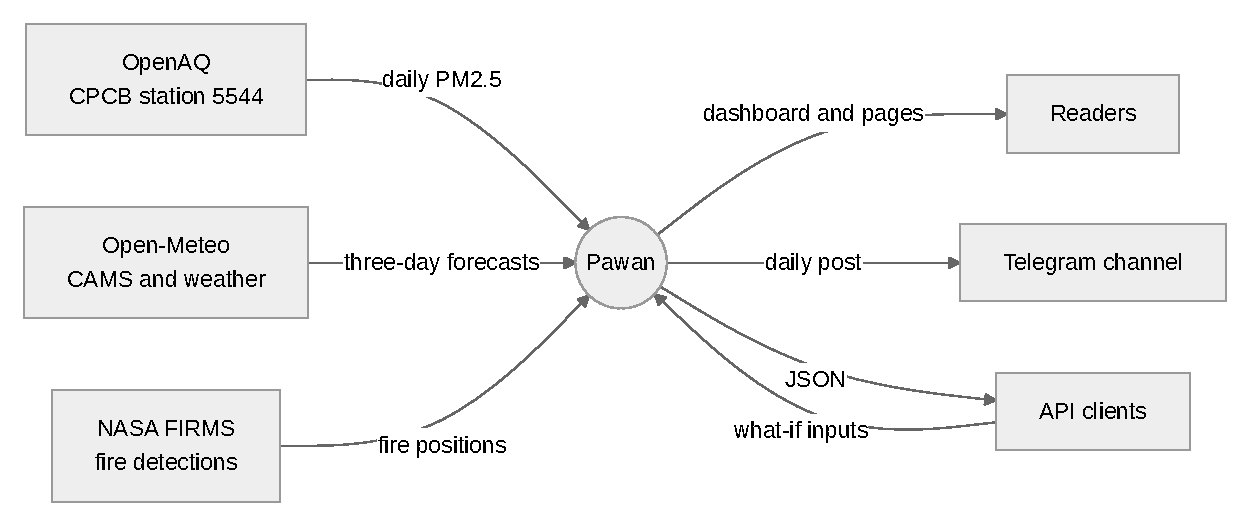
\includegraphics[width=0.9\linewidth]{figures/context.pdf}
  \caption{Context diagram: the data sources Pawan reads and the
    people and programs it serves}
  \label{fig:context}
\end{figure}

Figure~\ref{fig:dataflow} shows how data moves through the seven
processes of a daily run. Every data store is a file in the
repository. The daily table, \texttt{daily.csv}, is the only store
of observations; every other file is derived from it and can be
rebuilt.

\begin{figure}[htbp]
  \centering
  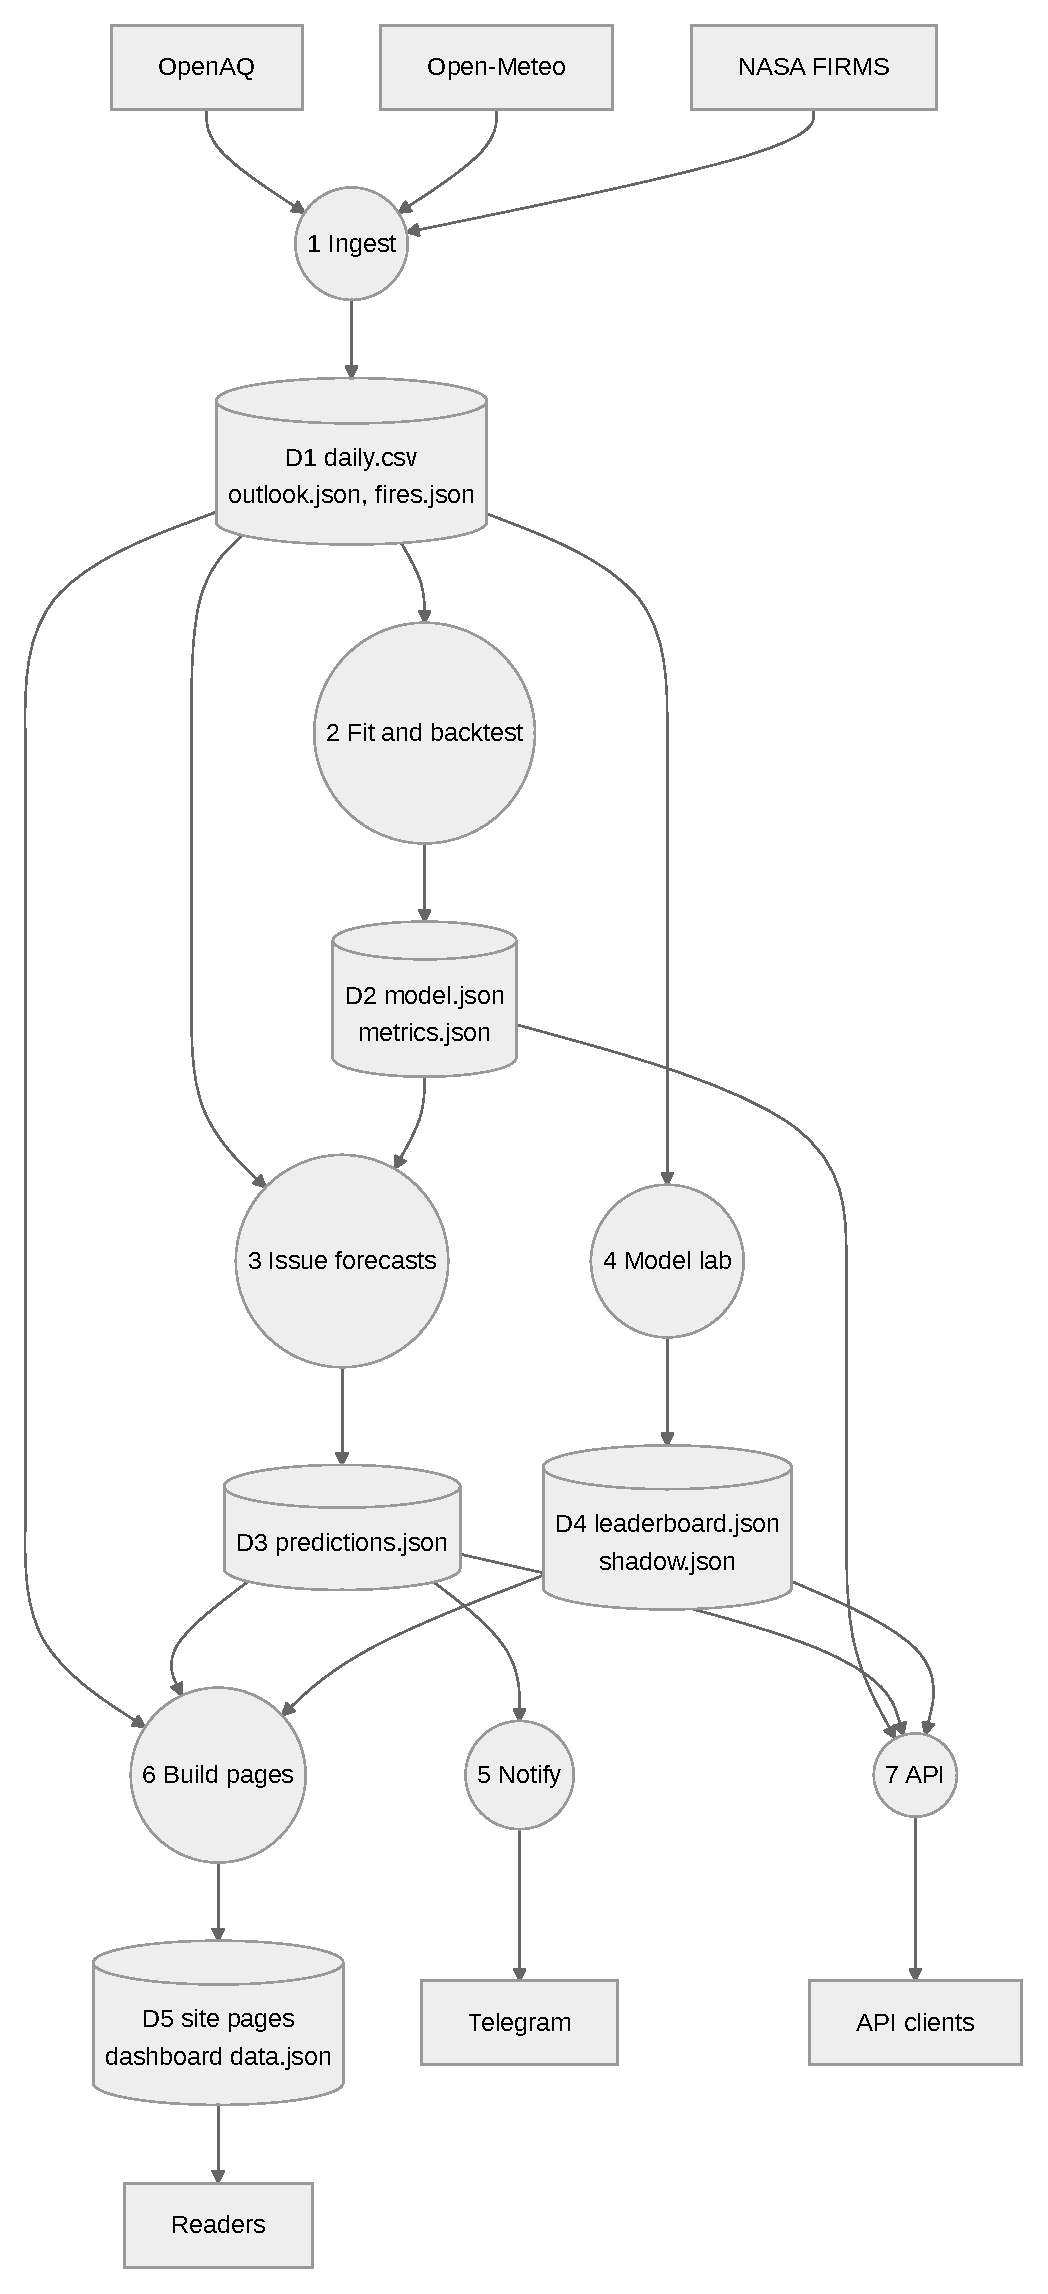
\includegraphics[width=0.62\linewidth]{figures/dataflow.pdf}
  \caption{Data flow diagram (level 1). Processes are numbered in
    the order the daily run performs them.}
  \label{fig:dataflow}
\end{figure}

Figure~\ref{fig:usecase} shows who uses the system and for what.
Readers view the forecast, try other inputs and compare models;
programs query the API; the scheduler runs the pipeline. Promoting a
new model is deliberately left to a person.

\begin{figure}[htbp]
  \centering
  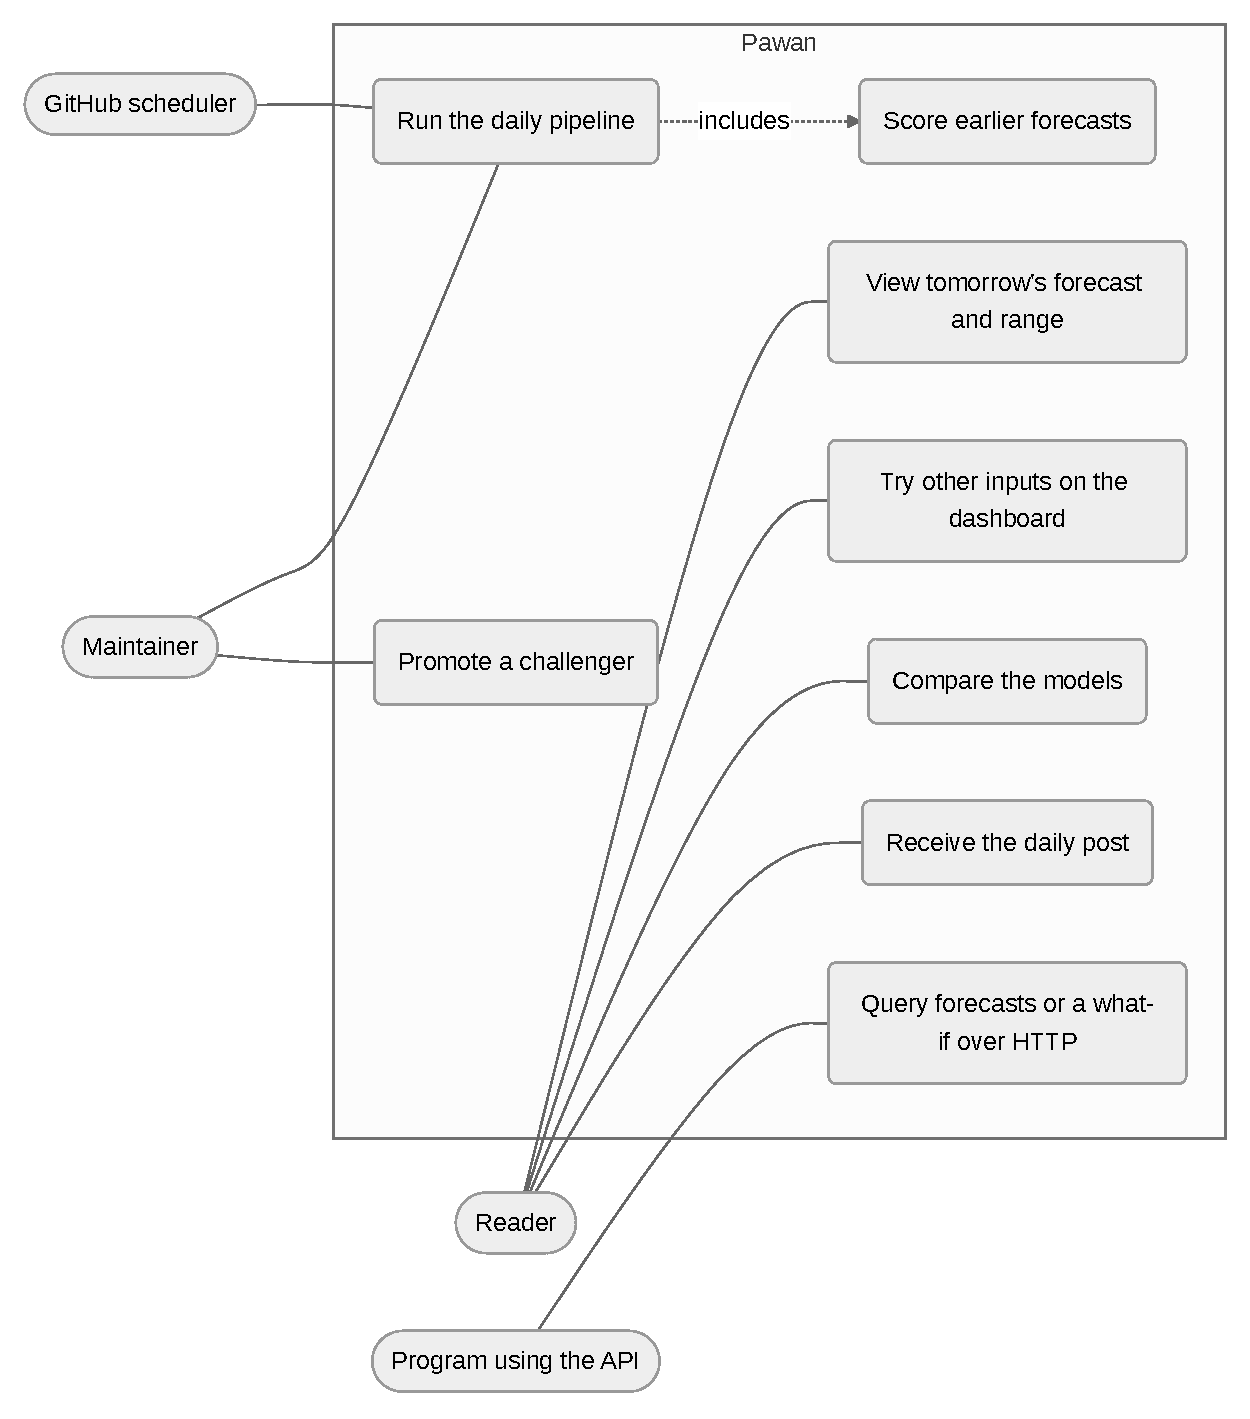
\includegraphics[width=0.75\linewidth]{figures/usecase.pdf}
  \caption{Use case diagram}
  \label{fig:usecase}
\end{figure}

Figure~\ref{fig:deployment} shows where each part runs. The pipeline
runs on GitHub's hosted runners, the site is static files on GitHub
Pages, and the API runs wherever the repository is cloned.

\begin{figure}[htbp]
  \centering
  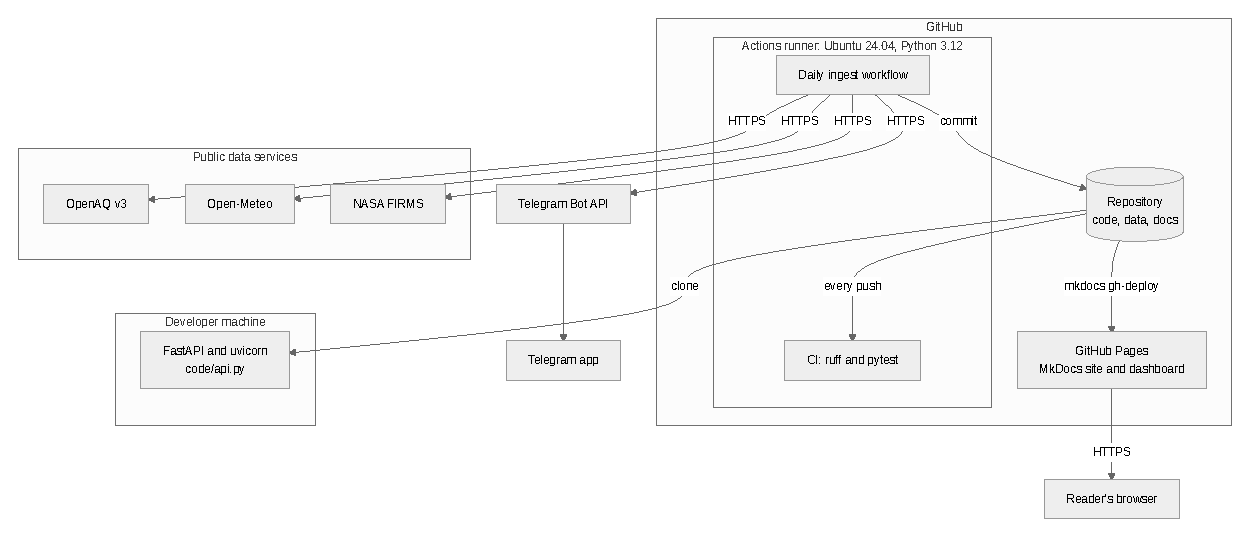
\includegraphics[width=0.95\linewidth]{figures/deployment.pdf}
  \caption{Deployment diagram}
  \label{fig:deployment}
\end{figure}

\subsection{Technical Stack}

\begin{itemize}
  \item \textbf{Framework/Language:} Python 3.12. The forecast path
    (ingestion, features, model, evaluation, pages) uses only the
    Python standard library, so it cannot break on a dependency
    upgrade. The dashboard is plain HTML, CSS and JavaScript.
  \item \textbf{Database:} none. The data is a CSV file of a few
    hundred rows committed to git, plus JSON files derived from it.
    The commit history is a complete record of every change to the
    data.
  \item \textbf{Tools:} GitHub Actions for the daily run and for
    continuous integration, GitHub Pages for hosting, pytest for
    testing, ruff for linting, MkDocs with Material for the project
    site \cite{mkdocsmaterial}, Mermaid for diagrams, and \LaTeX{}
    with the \texttt{tietreport} class for reports \cite{tietreport}.
  \item \textbf{Libraries:} scikit-learn for the benchmark models
    in the model lab \cite{pedregosa2011}, FastAPI and uvicorn for
    the API \cite{fastapi}, Leaflet for the fire map, and matplotlib
    for the report's charts. All are pinned to exact versions and
    kept out of the forecast path.
  \item \textbf{Data sources:} the CPCB station at Model Town,
    Patiala, through the OpenAQ v3 API \cite{openaq}; CAMS
    \pmtf{} forecasts and weather forecasts from Open-Meteo
    \cite{openmeteo}; fire detections from NASA FIRMS (VIIRS)
    \cite{firms,schroeder2014}. All are free and public.
  \item \textbf{Alerts:} the Telegram Bot API, for the daily post.
\end{itemize}

\section{Implementation Details}

\subsection{Module 1: Data Ingestion}

The ingestion script (\texttt{code/ingest/run\_daily.py}) runs
first each day. It fetches the last 30 days of daily station
readings, the CAMS and weather forecasts for the next three days,
and the previous day's fire detections in a box around Punjab and
Haryana, then merges them into \texttt{daily.csv} by date.

Three rules keep the table trustworthy.
\begin{itemize}
  \item \textbf{Validity.} A station day counts only if it is built
    from at least 16 hourly readings, the CPCB rule for a valid
    daily mean. Thinner days are kept but never used for training or
    scoring.
  \item \textbf{Staleness tripwire.} If the newest station reading
    is more than seven days old, the run fails loudly. This rule was
    added after a multi-week outage in which the job called the
    wrong API endpoint and kept reporting success.
  \item \textbf{Resilient requests.} Each request is retried. A
    server fault waits 2 and then 4 seconds; a busy source (HTTP
    429) or a stalled connection waits 15 and then 30 seconds, or as
    long as the source asks, up to a minute. Error messages remove
    API keys from URLs before printing them, because the logs of a
    public repository are public.
\end{itemize}

\subsection{Module 2: Feature Construction}

\texttt{code/features.py} turns each row of the table into the
inputs for one forecast. A forecast for day $D$ is issued on day
$D-1$, so every input must be known by then.

\begin{table}[htbp]
\centering
\small
\begin{tabular}{|l|L{8.6cm}|}
  \hline
  \textbf{Input} & \textbf{Definition} \\
  \hline
  \texttt{cams\_log} & $\log(1 + c)$, where $c$ is the CAMS
    forecast of the daily mean for day $D$ \\
  \hline
  \texttt{obs\_recent\_log} & $\log(1 + r)$, where $r$ is the
    freshest valid station reading, $a$ days before $D$ \\
  \hline
  \texttt{burning} & 1 in October and November, otherwise 0 \\
  \hline
  \texttt{temp}, \texttt{rh} & Forecast mean temperature and
    relative humidity for day $D$ \\
  \hline
  \texttt{wind\_speed} & Forecast mean wind speed for day $D$ \\
  \hline
  \texttt{wind\_u}, \texttt{wind\_v} & East and north wind
    components, so that 359\textdegree{} and 1\textdegree{} are
    treated as close \\
  \hline
  \texttt{fire\_log} & $\log(1 + n)$, where $n$ is the number of
    fires detected the day before the issue day \\
  \hline
\end{tabular}
\caption{The nine model inputs}
\label{tab:features}
\end{table}

The \emph{reading age} $a$ is central to the design. The station's
publication delay has changed over the semester: about three days
in August, irregular batches in early October, and about one day
since late October. Instead of assuming a fixed delay, the system
finds the freshest valid reading on file each morning and uses a
model fitted on readings of exactly that age, from two to seven
days. A model fitted on two-day-old readings has learnt how much a
two-day-old reading is worth, and is never given a five-day-old
one.

The fire count is taken from the day before the issue day, because
detections are recorded against the day they happen, and the issue
day's own count is not complete when the forecast goes out.
Figure~\ref{fig:datamodel} shows the data model.

\begin{figure}[htbp]
  \centering
  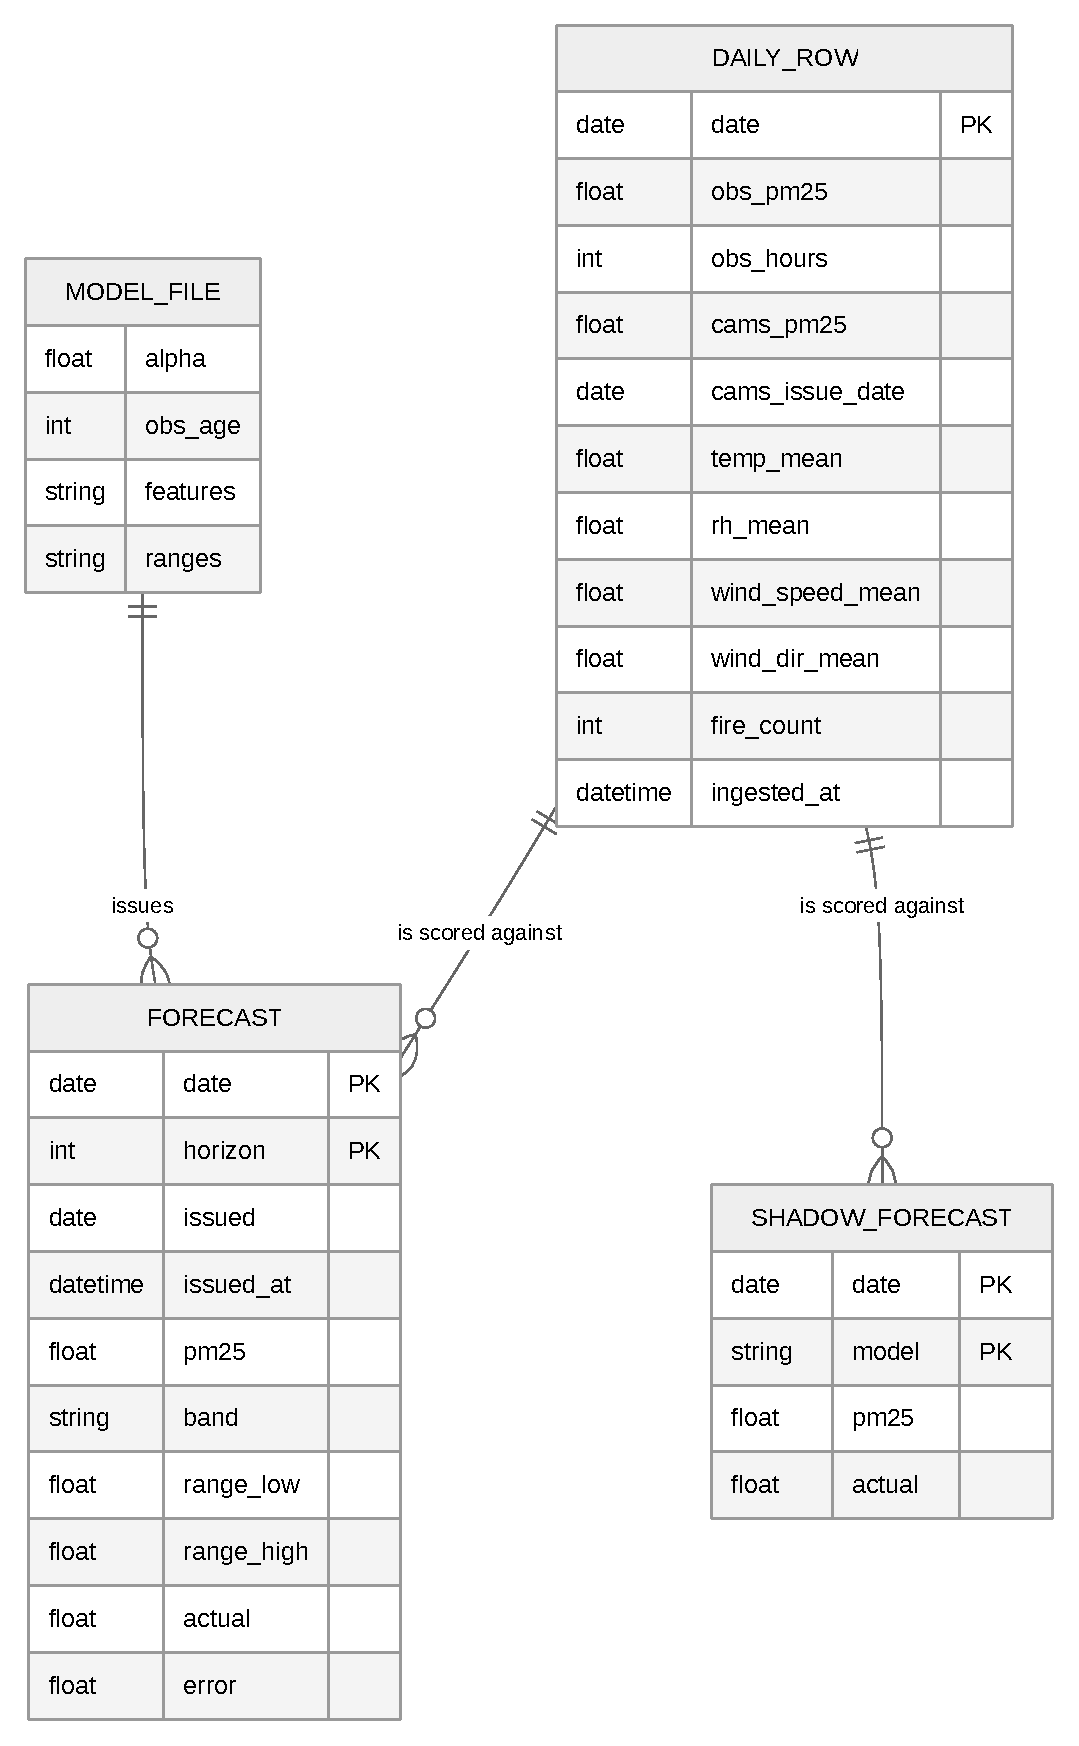
\includegraphics[width=0.8\linewidth]{figures/datamodel.pdf}
  \caption{Data model: the daily row, the forecast records and the
    model file}
  \label{fig:datamodel}
\end{figure}

\subsection{Module 3: Forecasting Model}

The shipped model is ridge regression \cite{hoerl1970} on the log
of the daily mean:
\[
  \log\left(1 + \hat{y}_D\right) = \beta_0 + \sum_{j} \beta_j\, z_{D,j},
\]
\[
  \hat{\beta} = \arg\min_{\beta} \sum_{t}
  \left(\log(1 + y_t) - \beta_0 - \beta^\top z_t\right)^2
  + \alpha \lVert \beta \rVert^2,
\]
where $z$ are the standardised inputs. Working in log space fits a
quantity that ranges from about 2 to over 140~\ugm{} and turns
the multiplicative effects of smoke into additive ones. The penalty
$\alpha$ is chosen from a grid by validation on the most recent
fifth of the training rows. The model is written by hand in about
200 lines of standard-library Python, so the dashboard can show
exactly how each input moved tomorrow's number.

Each forecast comes with a \emph{likely range}, sized so that four
days in five should fall inside it. The range is the middle 80\% of
the backtest's own out-of-sample errors in log space, taken
separately for the calm and burning seasons. Because the errors are
in log space, the range is wider above the forecast than below it,
which suits a quantity that rises in spikes.

\subsection{Module 4: Issuing and Scoring Forecasts}

\texttt{code/predict.py} issues tomorrow's forecast and the two days
after it, the three-day outlook. Each forecast is frozen when it is
issued: written once to \texttt{predictions.json} and never changed
by a later run. When the station publishes a valid reading for that
day, the measurement and the error are attached to the record.
Figure~\ref{fig:lifecycle} shows the states a forecast passes
through. Because forecasts cannot be revised, the live track record
shows what was actually claimed.

\begin{figure}[htbp]
  \centering
  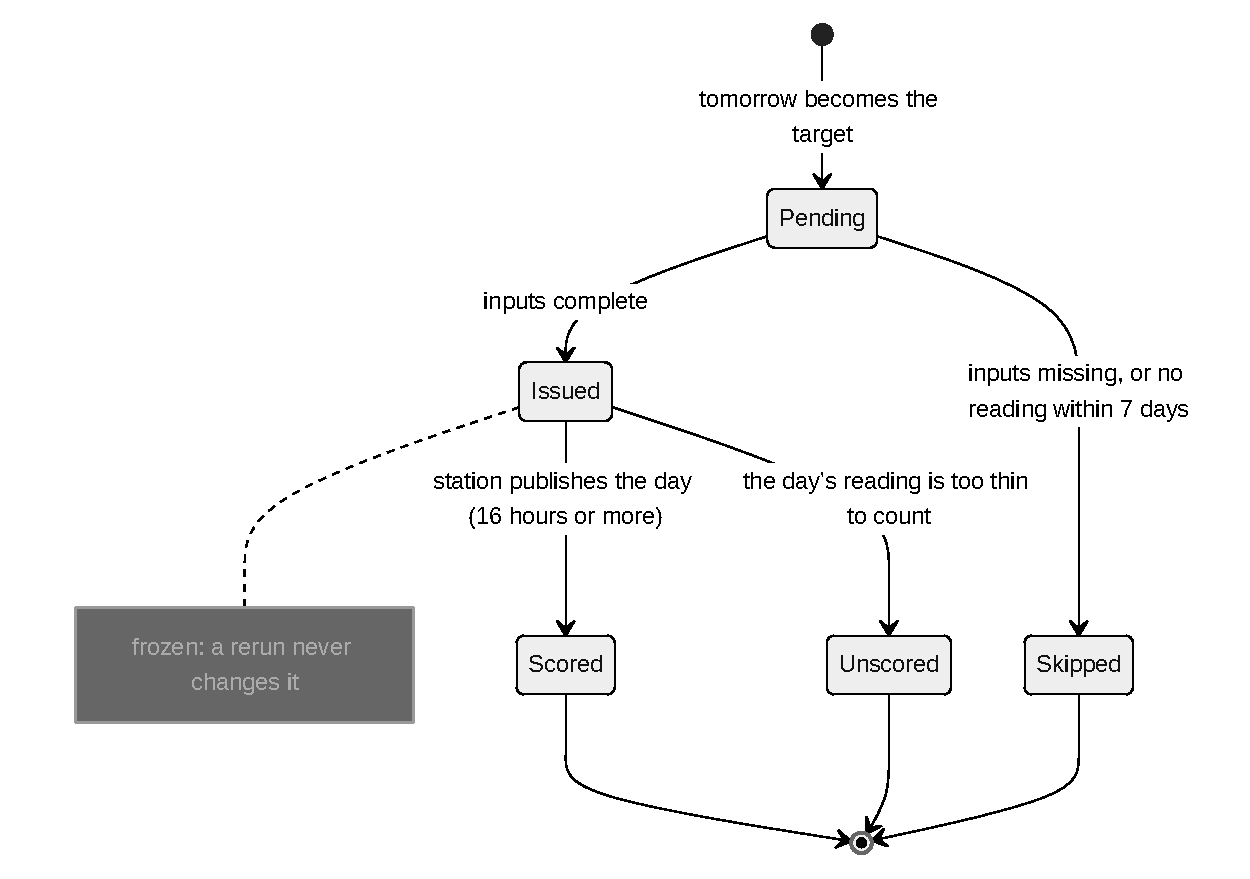
\includegraphics[width=0.62\linewidth]{figures/lifecycle.pdf}
  \caption{State diagram of a forecast record}
  \label{fig:lifecycle}
\end{figure}

\subsection{Module 5: Model Lab}

\texttt{code/candidates.py} and \texttt{code/lab.py} compare the
shipped model with eleven alternatives under identical rules: the
same days, the same reading for each forecast, and training data
that stops at the last day published before each forecast. The
candidates are three baselines (persistence, climatology, raw CAMS),
CAMS rescaled by its recent ratio to the station, ridge with
burning-season interaction terms, ridge corrected by its own errors
over the past week, an analog model that averages the most similar
past days, a random forest, gradient boosting, a small neural
network and an ensemble. Figure~\ref{fig:classes} shows the class
structure: every candidate implements the same \texttt{fit} method,
so the lab can treat them alike.

\begin{figure}[htbp]
  \centering
  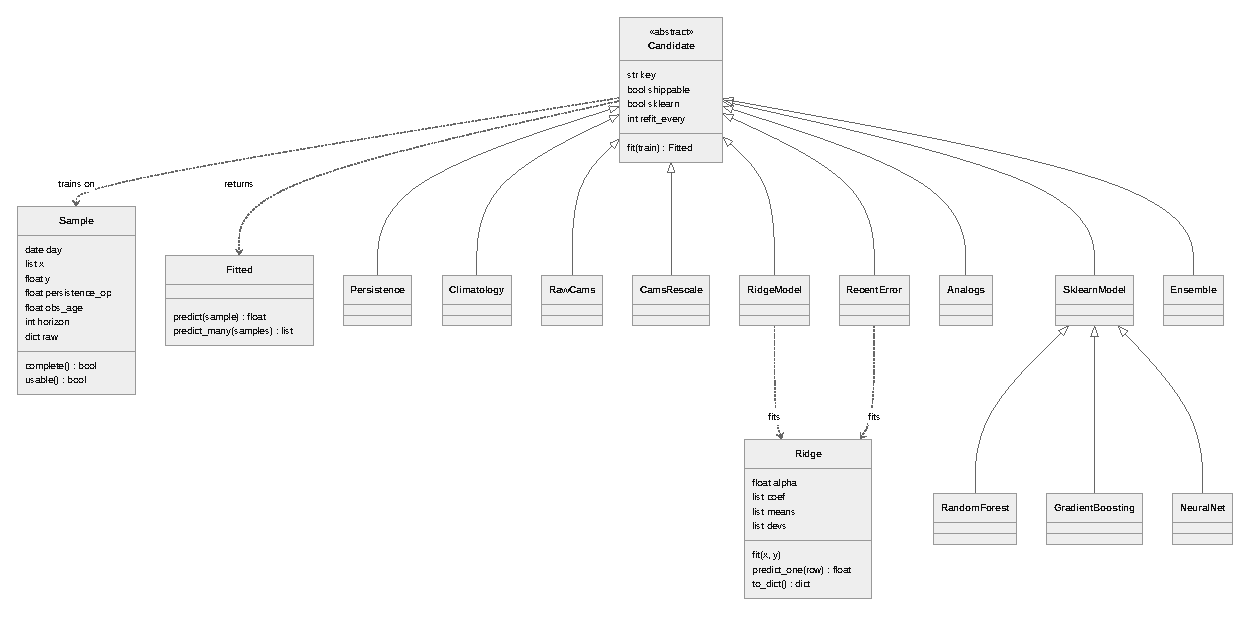
\includegraphics[width=\linewidth]{figures/classes.pdf}
  \caption{Class diagram of the model lab}
  \label{fig:classes}
\end{figure}

Every morning each candidate also issues a shadow forecast, which is
frozen and scored like the real one, so each model builds a live
record. A challenger replaces the shipped model only if it passes a
rule written in the code before the comparison was run: at least
\RuleBurnGain{} points of skill better in the burning season, no
more than \RuleCalmCost{} points worse in the calm season, within
\RuleRobust\% of the shipped model's error at every reading age from
two to five days, and no worse over \RuleLiveDays{} live days.
Promotion is then a one-line change made by a person in a pull
request.

\subsection{Module 6: Website and Dashboard}

\texttt{code/pages.py} rebuilds the public site from the data
files after every run. The dashboard (Figures~\ref{fig:dashhero}
to~\ref{fig:dashwhy}) shows tomorrow's forecast on the national AQI
scale next to the raw CAMS figure, the likely range, the next two
days, a map of yesterday's fires with tomorrow's wind, an exact
breakdown of what moved the forecast, sliders to try other inputs,
the past days that looked most like tomorrow, the full history,
and the model comparison. The sliders rerun the model in the
browser; before they are enabled, the page checks that its
arithmetic reproduces the forecast issued by the pipeline.

\begin{figure}[htbp]
  \centering
  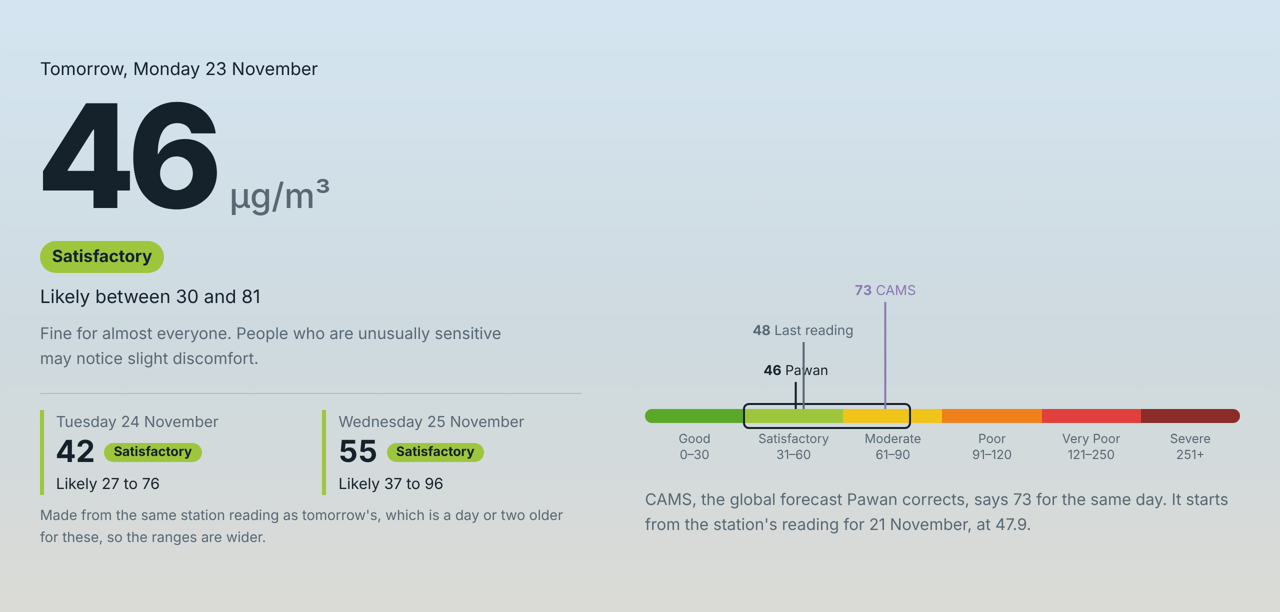
\includegraphics[width=\linewidth]{figures/dash-hero.png}
  \caption{Dashboard: tomorrow's forecast, its likely range and the
    next two days, on the national AQI scale}
  \label{fig:dashhero}
\end{figure}

\begin{figure}[htbp]
  \centering
  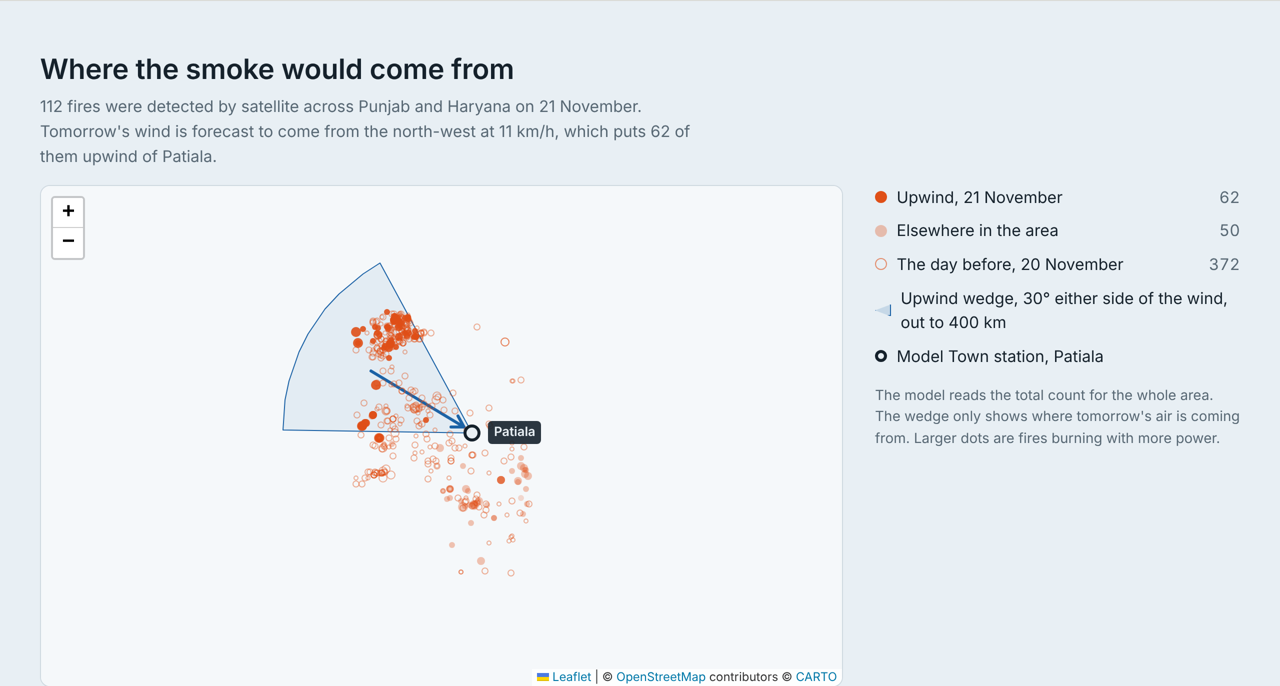
\includegraphics[width=\linewidth]{figures/dash-fires.png}
  \caption{Dashboard: fires detected the day before, and the upwind
    wedge for tomorrow's wind (map tiles omitted in this capture)}
  \label{fig:dashfires}
\end{figure}

\begin{figure}[htbp]
  \centering
  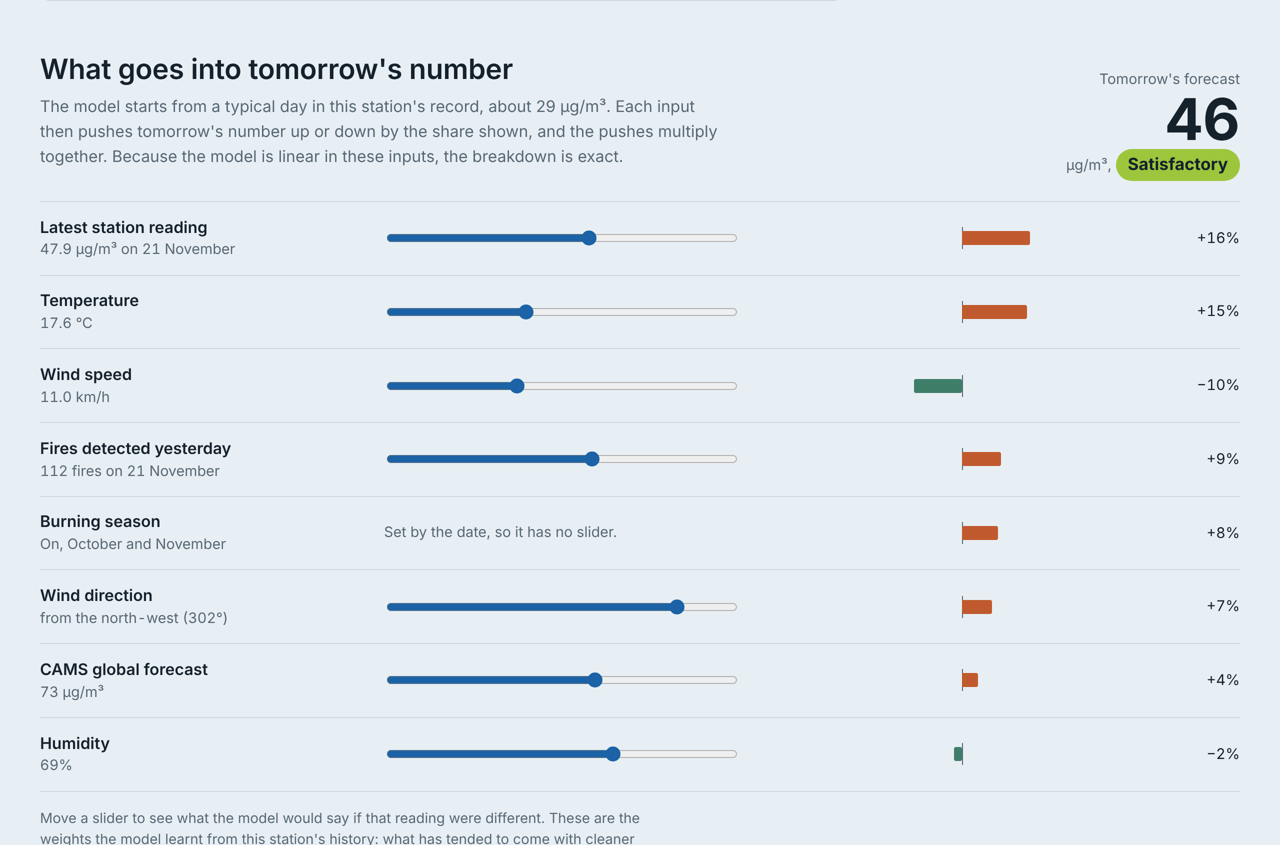
\includegraphics[width=\linewidth]{figures/dash-why.png}
  \caption{Dashboard: how each input moved tomorrow's forecast,
    with sliders to try other values}
  \label{fig:dashwhy}
\end{figure}

\subsection{Module 7: HTTP API}

\texttt{code/api.py} is a small FastAPI service \cite{fastapi} that
serves the same data to other programs. FastAPI generates the
interactive documentation in Figure~\ref{fig:api} from the code's
type annotations. The site does not depend on the API.

\begin{table}[htbp]
\centering
\small
\begin{tabular}{|l|l|L{8.2cm}|}
  \hline
  \textbf{Method} & \textbf{Path} & \textbf{Returns} \\
  \hline
  GET & \texttt{/forecast} & Tomorrow's forecast, range and advice,
    the next two days, or the reason there is no forecast \\
  \hline
  GET & \texttt{/forecasts} & Every forecast on record with its
    outcome; filters by date and by scoring \\
  \hline
  GET & \texttt{/models} & The model lab's comparison \\
  \hline
  GET & \texttt{/health} & Age of the newest reading and whether
    the feed is stale \\
  \hline
  POST & \texttt{/whatif} & The shipped model's forecast for
    supplied inputs \\
  \hline
\end{tabular}
\caption{API endpoints}
\label{tab:api}
\end{table}

The what-if endpoint refuses impossible inputs (for example,
humidity above 100\%) with an HTTP 422 response. It answers inputs
that are possible but outside anything the model was fitted on, and
lists them in its reply with the range that was seen in training.
The model file stores these ranges for that purpose.

\begin{figure}[htbp]
  \centering
  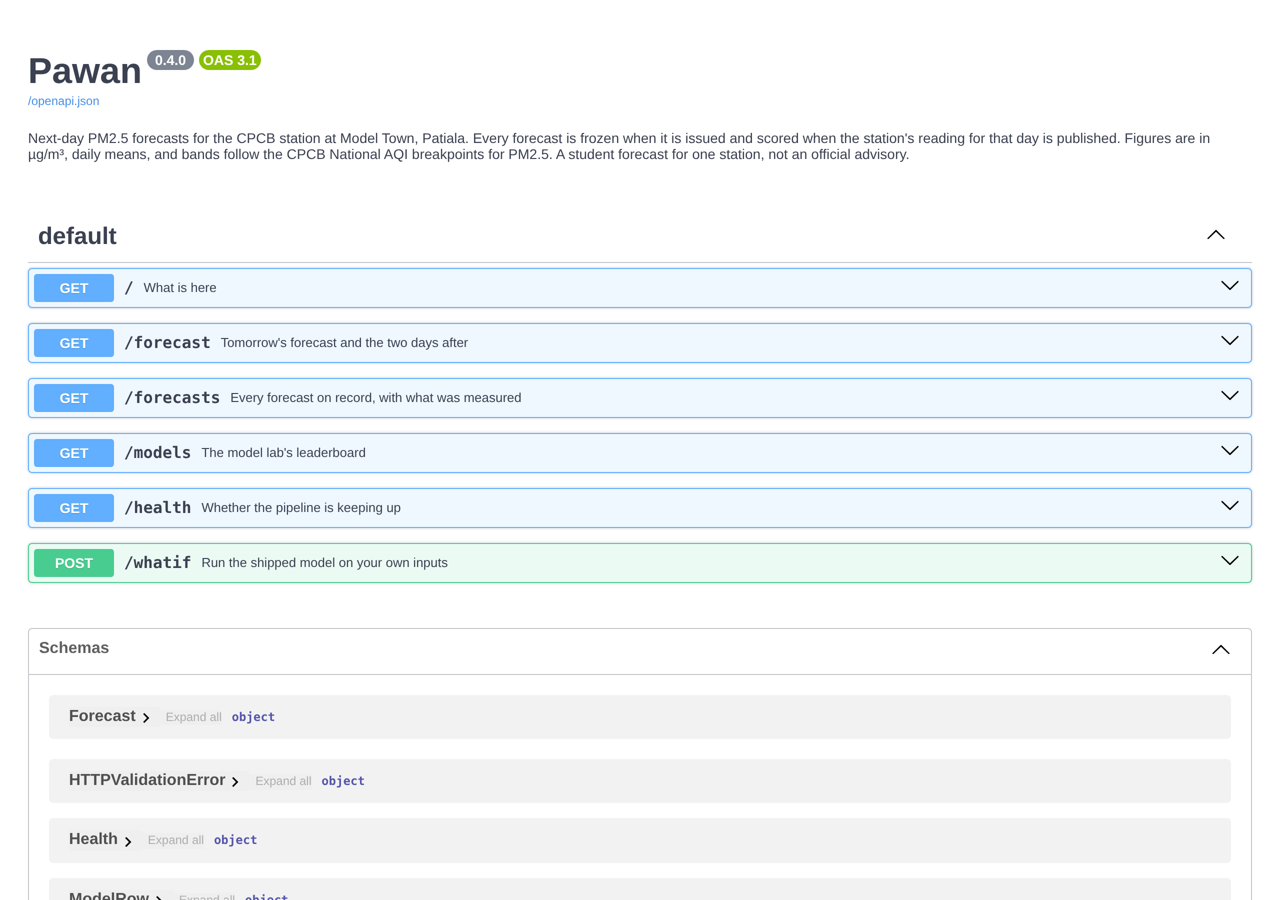
\includegraphics[width=0.95\linewidth]{figures/api-docs.png}
  \caption{Interactive API documentation generated by FastAPI}
  \label{fig:api}
\end{figure}

\subsection{Module 8: Alerts}

\texttt{code/notify.py} posts each day's forecast to a Telegram
channel: the number, the band, the likely range, advice for the
band and the next two days. A Poor or worse forecast leads with a
warning line, and a day without a forecast posts the reason instead
of nothing. Each forecast is posted once, however many times the
workflow runs. The bot token travels in the request URL, so the
module never prints a URL in an error message.

\subsection{Module 9: Automation and Scheduling}

The daily workflow is scheduled for 08:00 IST. Figure~\ref{fig:sequence}
shows one run. Steps after the data collection run even if an earlier
step failed, and the test suite runs before every commit, so a bad
day still keeps whatever data it collected. GitHub starts scheduled
runs late, often by several hours, so four backup runs follow
through the day. A small first job (\texttt{code/due.py}) lets a
backup do the work only if that day's run has already gone out
without a forecast, or if it is evening and there is no sign of a
run at all. A separate workflow runs the linter and the full test
suite on every pull request, and a third rebuilds the website on
every change to the main branch.

\begin{figure}[htbp]
  \centering
  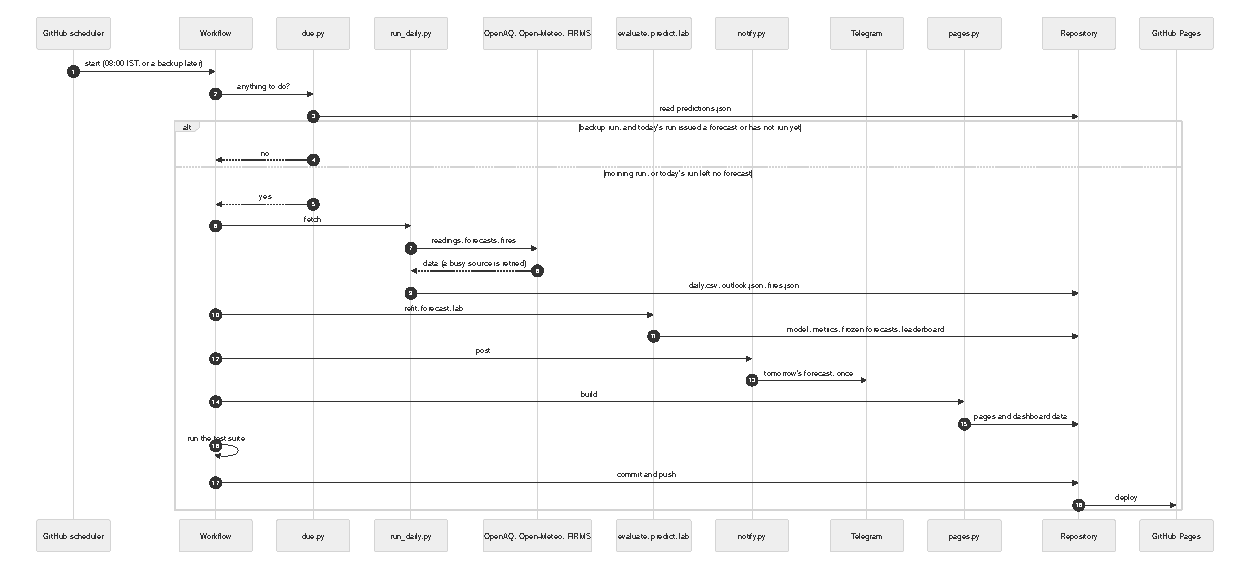
\includegraphics[width=\linewidth]{figures/sequence.pdf}
  \caption{Sequence diagram of a daily run}
  \label{fig:sequence}
\end{figure}

% ===== CHAPTER 3: RESULTS & EVALUATION =====

\chapter{Results and Evaluation}
\label{ch:results}

\section{Testing Methodology}

\begin{itemize}
  \item \textbf{Unit Testing:} \TestTotal{} automated tests in
    \TestFiles{} files cover each module (Table~\ref{tab:tests}).
    They include tests written for each failure found during the
    project, such as a backtest step that could see unpublished
    days, a backup run that could beat the morning run, and an error
    message that could print part of an API key.
  \item \textbf{Integration Testing:} the full suite runs on every
    pull request and again inside every daily run, before anything
    is committed. Each change in this report was also applied to a
    fresh copy of the repository and run through the whole daily
    pipeline on real data before it was merged.
  \item \textbf{Performance Testing:} forecast accuracy is measured
    by a walk-forward backtest \cite{hyndman2021}. The model is
    refitted for every day from \BtFirst{} to \BtLast, using only
    rows published before that day, and its error is compared with
    persistence given the same reading. Skill is the reduction in
    mean absolute error relative to persistence, in the spirit of
    the skill scores of \cite{murphy1988}. Running time was measured
    for the daily workflow and for the API.
  \item \textbf{User Testing:} no formal user study was carried out.
    Acceptance evidence comes from two sources: the prototype review
    in October, whose feedback on format and visible output shaped
    the second half of the project, and the live record, in which
    every forecast is scored against the measurement it predicted.
\end{itemize}

\begin{table}[htbp]
\centering
\small
\begin{tabular}{|l|r|}
  \hline
  \textbf{Test file} & \textbf{Tests} \\
  \hline
  \rows{data/tests.tex}
  \hline
  \textbf{Total} & \textbf{\TestTotal} \\
  \hline
\end{tabular}
\caption{Automated tests by file}
\label{tab:tests}
\end{table}

\section{Performance Metrics}

Table~\ref{tab:performance} compares the targets with the results.

\begin{table}[htbp]
\centering
\begin{tabular}{|l|r|r|}
  \hline
  \textbf{Metric} & \textbf{Target} &
  \textbf{Achieved} \\
  \hline
  Calm-season skill vs persistence & $\geq 10\%$ & \SkillCalm \\
  \hline
  Burning-season skill (two-day readings) & $\geq 20\%$ & \SkillBurn \\
  \hline
  Burning-season skill (four-day readings) & $\geq 20\%$ & \BurnSkillFour \\
  \hline
  Likely range holds the measurement & 80\% & \RangeRate \\
  \hline
  Forecast in the right AQI band & -- & \BandHit \\
  \hline
  Days with a forecast on record & -- & \PipeRate \\
  \hline
  Hourly station readings received & -- & \DataAvailability \\
  \hline
  Daily run, median of the last 30 & -- & 31 s \\
  \hline
  API response time, median & -- & 1.3--3.1 ms \\
  \hline
\end{tabular}
\caption{Performance results summary}
\label{tab:performance}
\end{table}

\subsection{Accuracy against the baselines}

Table~\ref{tab:backtest} gives the backtest over \BtDays{} days with
two-day-old readings, the freshness the station now delivers.
Figure~\ref{fig:record} shows the whole period. Pawan has the lowest
error in both seasons. Raw CAMS misses by more than four times as
much as Pawan, and persistence is the strongest baseline.

\begin{table}[htbp]
\centering
\begin{tabular}{|l|r|r|r|r|}
  \hline
  \textbf{Period} & \textbf{Days} & \textbf{Pawan} &
  \textbf{Persistence} & \textbf{Raw CAMS} \\
  \hline
  Calm season & \DaysCalm & \MaeCalm & \PersCalm & \CamsCalm \\
  \hline
  Burning season & \DaysBurn & \MaeBurn & \PersBurn & \CamsBurn \\
  \hline
  All days & \BtDays & \MaePawan & \MaePers & \MaeCams \\
  \hline
\end{tabular}
\caption{Mean absolute error in \ugm, walk-forward backtest,
  \BtFirst{} to \BtLast}
\label{tab:backtest}
\end{table}

\begin{figure}[htbp]
  \centering
  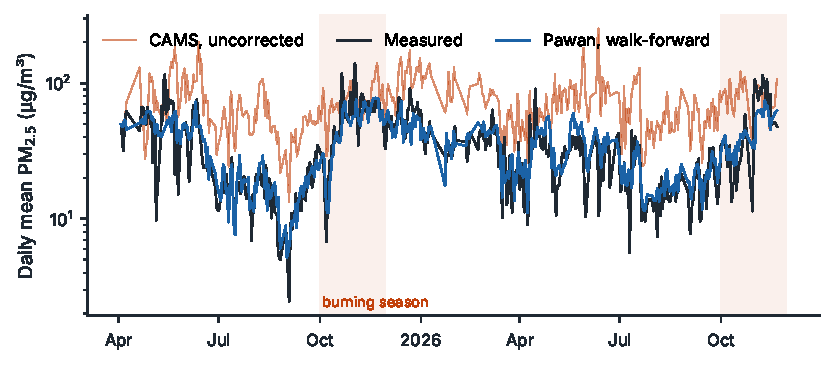
\includegraphics[width=\linewidth]{figures/record.pdf}
  \caption{Measured daily mean, Pawan's walk-forward forecast and
    raw CAMS, on a log scale. Shaded: burning seasons.}
  \label{fig:record}
\end{figure}

\begin{figure}[htbp]
  \centering
  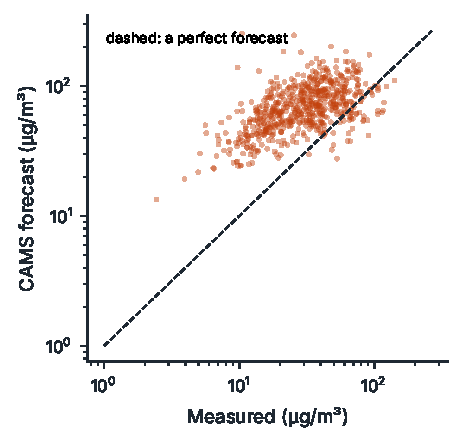
\includegraphics[width=0.48\linewidth]{figures/cams.pdf}
  \caption{CAMS forecast against the station's measurement. Most
    points lie well above the dashed line of a perfect forecast.}
  \label{fig:cams}
\end{figure}

\subsection{Effect of the reading age}

Table~\ref{tab:age} and Figure~\ref{fig:age} show the shipped model
at every reading age. Both errors grow as the reading gets older,
but persistence degrades faster, so Pawan's skill rises from
\SkillAll{} with a two-day-old reading to over 20\% with a four-day-old
one. When the targets were set in August, the freshest reading on
the issue day was four days old. The station has since become
faster, which makes the baseline stronger.

\begin{table}[htbp]
\centering
\small
\begin{tabular}{|l|r|r|r|r|r|r|}
  \hline
  \textbf{Reading age} & \textbf{Days} & \textbf{Pawan} &
  \textbf{Persistence} & \textbf{Skill} & \textbf{Calm} &
  \textbf{Burning} \\
  \hline
  \rows{data/by_age.tex}
  \hline
\end{tabular}
\caption{The shipped model at each reading age (MAE in \ugm)}
\label{tab:age}
\end{table}

\begin{figure}[htbp]
  \centering
  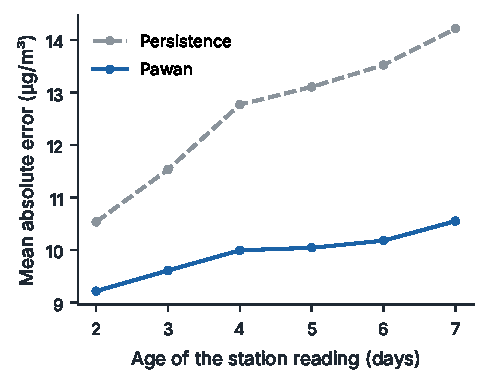
\includegraphics[width=0.55\linewidth]{figures/age.pdf}
  \caption{Error against the age of the station reading}
  \label{fig:age}
\end{figure}

\subsection{Model comparison}

Table~\ref{tab:leaderboard} and Figure~\ref{fig:leaderboard} give
the model lab's comparison of \LabModels{} models on the same
\LabDays{} days, run on \LabDate. The shipped ridge model
(\LabShippedMae) is ahead of every non-linear model; the best of
them, the \MakeLowercase{\LabBestBenchmark}, scores
\LabBestBenchmarkMae. Two ridge variants score slightly lower than
the shipped model, but neither passes the promotion rule: the smoke
terms break down with older readings, and the recent-error
correction gains less than \RuleBurnGain{} points in the burning
season. Both continue to be scored live.

\begin{table}[htbp]
\centering
\footnotesize
\begin{tabular}{|l|l|r|r|r|r|}
  \hline
  \textbf{Model} & \textbf{Kind} & \textbf{MAE} & \textbf{Skill} &
  \textbf{Burning} & \textbf{Live (days)} \\
  \hline
  \rows{data/leaderboard.tex}
  \hline
\end{tabular}
\caption{Model lab comparison, two-day-old readings. Skill is
  against persistence; Live is the mean absolute error of each
  model's shadow forecasts so far.}
\label{tab:leaderboard}
\end{table}

\begin{figure}[htbp]
  \centering
  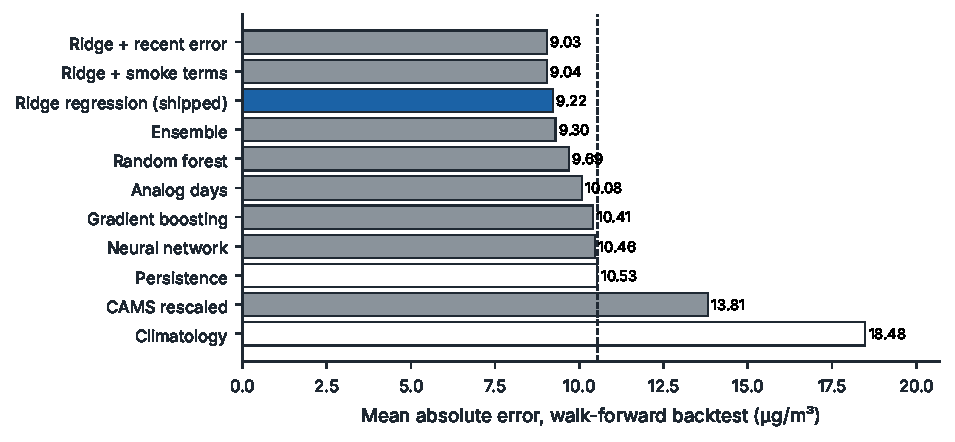
\includegraphics[width=0.9\linewidth]{figures/leaderboard.pdf}
  \caption{Backtest error by model. Blue: the shipped model;
    dashed line: persistence. Raw CAMS (\MaeCams) is left out of the
    chart for scale.}
  \label{fig:leaderboard}
\end{figure}

\subsection{Three-day outlook and the likely range}

Table~\ref{tab:outlook} gives the backtest for each horizon. Skill
over persistence grows with the horizon, because persistence falls
off faster. The likely range held the measurement on \RangeHeld{}
of \RangeDays{} backtest days (\RangeRate), against a target of 80\%,
and on \RangeBurnHeld{} of \RangeBurnDays{} burning-season days
(\RangeBurnRate). Since the range was resized in November, it has
held on \LiveRangeHeld{} of \LiveRangeDays{} live days. Before the
resize it held on about half of live days, because it was sized
from the fit's own errors.

\begin{table}[htbp]
\centering
\small
\begin{tabular}{|l|r|r|r|r|r|r|}
  \hline
  \textbf{Days ahead} & \textbf{Reading} & \textbf{Days} &
  \textbf{Pawan} & \textbf{Persistence} & \textbf{Skill} &
  \textbf{Range held} \\
  \hline
  \rows{data/outlook.tex}
  \hline
\end{tabular}
\caption{Backtest by forecast horizon (MAE in \ugm)}
\label{tab:outlook}
\end{table}

\subsection{Live record}

Since \LiveFirst, the system has issued \LiveIssued{} next-day
forecasts, of which \LiveScored{} have been scored against a valid
reading (Figure~\ref{fig:live}). Their mean absolute error is
\LiveMae~\ugm, against \LivePersMae~\ugm{} for persistence given the
same reading. The live period is short and includes the change of
reading age in November, so the backtest remains the main measure
of accuracy.

\begin{figure}[htbp]
  \centering
  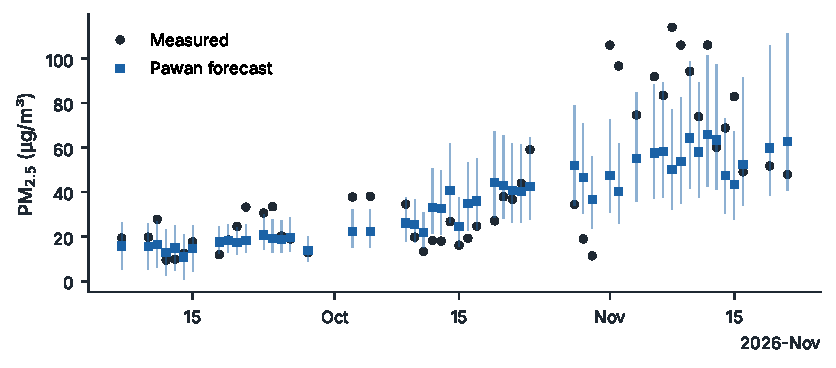
\includegraphics[width=\linewidth]{figures/live.pdf}
  \caption{Live forecasts and measurements. Vertical lines: the
    likely range, where one was issued.}
  \label{fig:live}
\end{figure}

\section{Analysis}

\begin{itemize}
  \item \textbf{Did the project meet its objectives?} Five of the
    eight objectives are met (Table~\ref{tab:objectives}). The
    calm-season target is met at every reading age. The
    burning-season target is met with the four-day-old readings it
    was set against, and not with today's fresher readings. The
    advisory objective is not met: the model has not forecast a
    Poor or worse day in advance, in the backtest (\PoorHit{} of
    \PoorDays) or live (\LivePoorHit{} of \LivePoorDays). It has also
    issued no false alarms (\PoorFalse), because it has not forecast
    above 90~\ugm{} in the backtest.
  \item \textbf{Where did it exceed expectations?} The system goes
    beyond the single dashboard in the proposal: it adds a
    three-day outlook, a calibrated range, a comparison of twelve
    models with live shadow forecasts, an HTTP API and daily alerts.
    The evaluation is stricter than planned. Forecasts are frozen
    when issued, and backtests follow the publication delay of the
    station.
  \item \textbf{What challenges were encountered?} The main ones
    were changes in the data sources and mistakes in the evaluation
    that made the results look better than they were.
    Table~\ref{tab:challenges} lists them with the risks named in
    the proposal.
  \item \textbf{How were they resolved?} Each was fixed in a pull
    request with a test that fails if the problem returns, and
    recorded in the weekly journal.
\end{itemize}

\begin{table}[htbp]
\centering
\small
\begin{tabular}{|L{3.4cm}|L{4.6cm}|L{4.8cm}|}
  \hline
  \textbf{Risk or problem} & \textbf{What happened} &
  \textbf{Resolution} \\
  \hline
  Silent interface failure (proposal) & The job called the wrong
  OpenAQ endpoint for weeks and still reported success &
  Correct endpoint; staleness tripwire fails the run after seven
  days without a reading \\
  \hline
  Temporal leakage (proposal) & The same-day fire count, and later
  a backtest that trained on unpublished days, overstated the
  accuracy & Lagged fire count; training stops at the last
  published day; tests for both \\
  \hline
  Station outage (proposal) & Gaps and thin days in the feed &
  16-hour validity rule; forecasts use the freshest valid reading
  and stop after seven days \\
  \hline
  Distribution shift at season onset (proposal) & Little
  burning-season history at first & History extended to February
  2025; seasons scored separately \\
  \hline
  Ambiguous station identity (proposal) & The station's original
  \pmtf{} sensor stopped reporting in 2022 & Live sensor identified
  and fixed in configuration \\
  \hline
  Changing publication delay & A fixed three-day lag discarded
  fresher readings once the station became faster & Freshest
  reading on file, with a model per reading age \\
  \hline
  Busy or unreachable weather API & Five failed runs between 15 and
  21 November & Longer retries; four backup runs through the day \\
  \hline
  Overfitted challenger & A smoke model forecast 2684~\ugm{} for a
  day that measured 13 & Promotion rule checks every reading age \\
  \hline
  Secret exposure & Error messages could print part of an API key
  in public logs & Keys removed before any URL is printed \\
  \hline
\end{tabular}
\caption{Risks, problems and how they were resolved}
\label{tab:challenges}
\end{table}

% ===== CHAPTER 4: CONCLUSION =====

\chapter{Conclusion}

\section{Summary of Work}

The project built and ran a complete forecasting system for one
station. It collects data every day without anyone running it,
issues a next-day forecast and a three-day outlook with likely
ranges, scores every forecast against the measurement, compares
twelve models under the same rules, and publishes the results on a
website, through an API and as a daily alert. The calm-season
accuracy target is met, the burning-season target is met at the
reading age it was set for, and the advisory target is not yet met.
Table~\ref{tab:milestones} gives the milestones, each delivered as
one or more reviewed pull requests.

\begin{table}[htbp]
\centering
\small
\begin{tabular}{|l|L{10.2cm}|}
  \hline
  \textbf{Date} & \textbf{Milestone} \\
  \hline
  29 Jul 2026 & Repository created from the course template \\
  \hline
  15--17 Aug & Daily data collection, continuous integration and
    baselines (PRs \#1--\#5) \\
  \hline
  6--7 Sep & Ingestion outage fixed, staleness tripwire, first
    daily forecast; week 3 and 4 journals (PRs \#6--\#11) \\
  \hline
  14 Sep & Model rework (weather inputs, log space, leak fixes) and
    the first forecast pages (PRs \#12--\#14) \\
  \hline
  10 Oct & Forecast gaps closed, burning-season history added,
    prototype report (PRs \#15--\#17); prototype review on 12 Oct \\
  \hline
  24 Oct & Live dashboard (PR \#18) \\
  \hline
  15 Nov & Freshest readings, model lab, outlook, calibrated range
    and alerts (PRs \#19, \#20 and \#22) \\
  \hline
  22 Nov & Retries and backup runs, recent-error challenger, HTTP
    API and design documentation (PRs \#23--\#25) \\
  \hline
\end{tabular}
\caption{Milestone log}
\label{tab:milestones}
\end{table}

\section{Key Findings}

\begin{itemize}
  \item \textbf{Finding 1:} The global forecast needs local
    correction at this station. Raw CAMS has an error of
    \MaeCams~\ugm; the corrected forecast has \MaePawan~\ugm.
  \item \textbf{Finding 2:} Persistence is the right benchmark, and
    its strength depends on the age of the reading. Skill claims
    are only meaningful when persistence is given the same reading
    as the model.
  \item \textbf{Finding 3:} On about 500 days of data, a regularised
    linear model beats a random forest, gradient boosting and a
    neural network under identical rules.
  \item \textbf{Finding 4:} Strict evaluation changes results. Two
    leaks found during the project each made the model look better
    than it was, and freezing forecasts made the live record
    trustworthy.
  \item \textbf{Finding 5:} The model does not anticipate pollution
    spikes. During smoky spells it stays low for days in a row, and
    its own recent errors are the clearest signal that a spell is
    under way.
\end{itemize}

\section{Future Work and Recommendations}

\begin{enumerate}
  \item Forecast spikes: promote the recent-error correction if it
    passes its live test, and add inputs that describe stagnant air,
    such as boundary layer height and a longer fire window.
  \item Forecast the probability of a Poor or worse day directly,
    so that the advisory can be judged by recall and false alarms.
  \item Store each day's CAMS and weather forecasts for every
    horizon, so the outlook can be backtested with the inputs it
    really had.
  \item Add more Punjab stations, such as Ludhiana, Amritsar and
    Bathinda. The station is a configuration value, so each new
    station is a new configuration entry and a new fit.
  \item Host the API publicly and carry out a short user study of
    the dashboard and the alerts, including a Punjabi or Hindi
    version of the page.
  \item Move the data to a database if the number of stations grows
    beyond a few.
\end{enumerate}

\section{Final Remarks}

The project shows that a small, transparent model can improve on a
global forecast at one station, provided it is judged against an
honest baseline with only the data available at the time. Most of
the engineering effort went into making that judgement reliable:
fixed rules for what each forecast may know, frozen records,
automated tests for every failure found, and a pipeline that keeps
running without supervision. The open problem, forecasting the worst
days in advance, is now clearly measured, and the system is set up
to test solutions to it every day.

% ===== BIBLIOGRAPHY =====

% Print bibliography with heading in TOC
\printbibliography[heading=bibintoc]

\end{document}
